Aplikasi Rugby Indonesia yang ada digunakan bagi para pemain rugby di Indonesia memiliki halaman utama yang berisi berita-berita terkini terkait permainan rugby yang ada di Indonesia, toolbar yang berisikan tombol home untuk kembali ke halaman utama, dan tombol menu untuk berpindah ke menu lainnya. Selain berfungsi untuk membaca berita, aplikasi yang ada ini berfungsi untuk menangkap gambar dan menguploadnya pada halaman teammate photo, melihat rugby clubs yang berada di tiap daerah, serta dapat melihat skor dari tiap pertandingan.

\begin{figure} [!h]
    \centering
    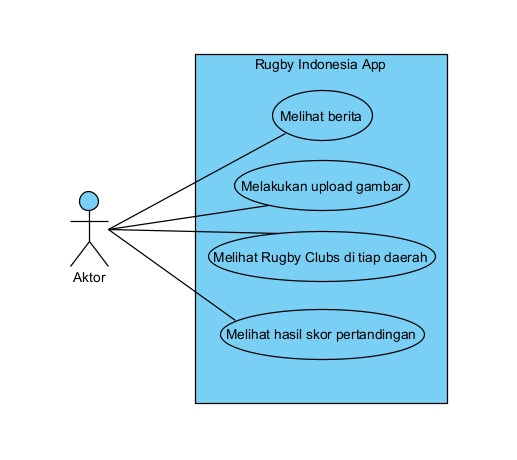
\includegraphics{Gambar/Existing-UCD-Rugby-App.png}
    \caption{Use Case Diagram Rugby Indonesia App}
    \label{fig:ucd-rugby-indonesia-app}
\end{figure}

\subsection{Halaman Utama}
Pada halaman Utama dari Rugby Indonesia, terdapat berita-berita terkini yang diambil dari halaman \url{rugbyindonesia.or.id/berita/}, tombol ``read more'' untuk melihat berita yang ingin dibaca lebih lengkap. Halaman ini merupakan halaman awal saat pengguna membuka aplikasi Rugby Indonesia pertama kali. 

\begin{table} [!h]
    \centering
    \caption{Tabel Skenario Awal dari Aplikasi Rugby Indonesia}
    \begin{tabular}{|c|c|c|}
    \hline
       No. & Aksi Aktor & Reaksi Sistem  \\ \hline
        1 & Membuka aplikasi & Aplikasi Rugby Indonesia menampilkan halaman \\
         & Rugby Indonesia & utama yang berisi berita Rugby Indoensia. \\ \hline
        2 & Pengguna mengklik & Aplikasi Rugby Indonesia akan menampilkan \\ 
         & tombol home &  halaman utama. \\ \hline
        3 & Pengguna mengklik & Aplikasi Rugby Indonesia akan menampilkan \\ 
         & tombol menu &  side menu yang berisi menu-menu dari \\ 
         & &  aplikasi Rugby Indonesia. \\ \hline
        4 & Pengguna mengklik & Aplikasi Rugby Indonesia akan menampilkan \\
          & tombol ``read more'' & berita yang dipilih oleh pengguna secara lengkap. \\ \hline
    \end{tabular}
    \label{tab:existing-scenario-welcome-page}
\end{table}

\subsection{Halaman Teammate Photos}

Pada halaman teammate photos, pengguna dapat melihat serta mengupload gambar maupun tangkapan gambar yang ingin diunggah ke dalam halaman ini. Pengguna juga dapat memberikan frame terhadap foto yang ingin diunggahnya.

\begin{table} [!h]
    \centering
    \caption{Tabel Skenario dari Halaman Teammate Photos}
    \begin{tabular}{|c|c|c|}
    \hline
       No. & Aksi Aktor & Reaksi Sistem  \\ \hline
        1 & Pengguna menekan tombol teammate & Aplikasi Rugby Indonesia menampilkan \\
         &  photos pada side menu. & halaman Teammate Photos \\ \hline
        2 & Pengguna mengklik & Aplikasi akan membuka camera \\ 
         & tombol ``take a photo'' &  \\ \hline
        3 & Pengguna mengklik & Aplikasi akan membuka  \\ 
         & tombol ``load from library'' & library gambar  \\ \hline
        4 & Pengguna mengklik & Aplikasi akan menampilkan \\
          & gambar yang ada & gambar tersebut lebih besar. \\ \hline
    \end{tabular}
    \label{tab:existing-scenario-teammate-photos-page}
\end{table}

\subsection{Halaman Rugby Clubs}
Pada halaman rugby clubs, pengguna dapat melihat informasi terkait klub rugby yang berada di tiap daerah

\begin{table} [!h]
    \centering
    \caption{Tabel Skenario dari Halaman Rugby Clubs}
    \begin{tabular}{|c|c|c|}
    \hline
       No. & Aksi Aktor & Reaksi Sistem  \\ \hline
        1 & Pengguna menekan tombol rugby & Aplikasi Rugby Indonesia menampilkan \\
         &  clubs pada side menu. & halaman Rugby Clubs \\ \hline
    \end{tabular}
    \label{tab:existing-scenario-rugby-clubs-page}
\end{table}

\subsection{Halaman Fixture \& Results}
Pada halmaan Fixture \& Results, pengguna dapat melihat hasil pertandingan skor dari permainan rugby yang sudah diselenggarakan.

\begin{table} [!h]
    \centering
    \caption{Tabel Skenario dari Halaman Fixture \& Results}
    \begin{tabular}{|c|c|c|}
    \hline
       No. & Aksi Aktor & Reaksi Sistem  \\ \hline
        1 & Pengguna menekan tombol Fixture & Aplikasi Rugby Indonesia menampilkan \\
         & \& Results pada side menu. & halaman Fixture \& Results \\ \hline
        2 & Pengguna mengklik salah & Aplikasi akan memperlihatkan \\ 
         & satu pertandingan yang ada & skor dari hasil pertandingan tersebut \\ \hline
    \end{tabular}
    \label{tab:existing-scenario-fixture-results-page}
\end{table}

Aplikasi Rugby Indoensia saat ini menggunakan framework Ionic versi 3, Apache Cordova, dan Angular. Aplikasi ini memungkinkan untuk ditulis menggunakan bahasa pemrograman seperti HTML, CSS, dan JavaScript.

\section{Analisis Sistem Usulan}
Aplikasi Rugby Indonesia yang akan dibangun hampir sama seperti aplikasi dengan sistem terkini, namun dengan tidak adanya halaman Fixture \& Results, Rugby Clubs dan fitur Push Notification dikarenakan website dari Rugby Indonesia sendiri yang sudah dipangkas sehingga tidak memiliki halaman-halaman tersebut.

\begin{figure} [!h]
    \centering
    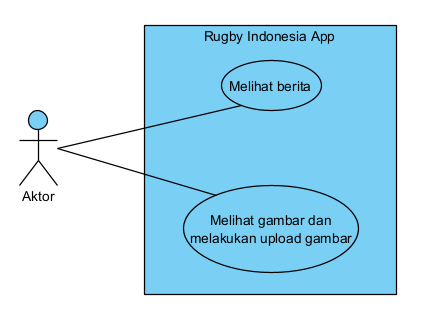
\includegraphics{Gambar/UCD-Proposal-Rugby-App.png}
    \caption{UCD Sistem Usulan Rugby Indonesia}
    \label{fig:proposal-ucd-rugby-indonesia}
\end{figure}

\subsection{Halaman Utama}
Pada halaman utama, skenario dari penggunaan aplikasi Rubgy Indoensia pada halaman utama sama seperti tabel skenario halaman utama dari sistem terkini [\ref{tab:existing-scenario-welcome-page}]. Halaman ini memiliki beberapa komponen yang terdapat pada Ionic 7, komponen-komponen yang terdapat pada halaman utama ini yaitu komponen toolbar, content, serta card. 

\begin{figure} [H]
    \centering
    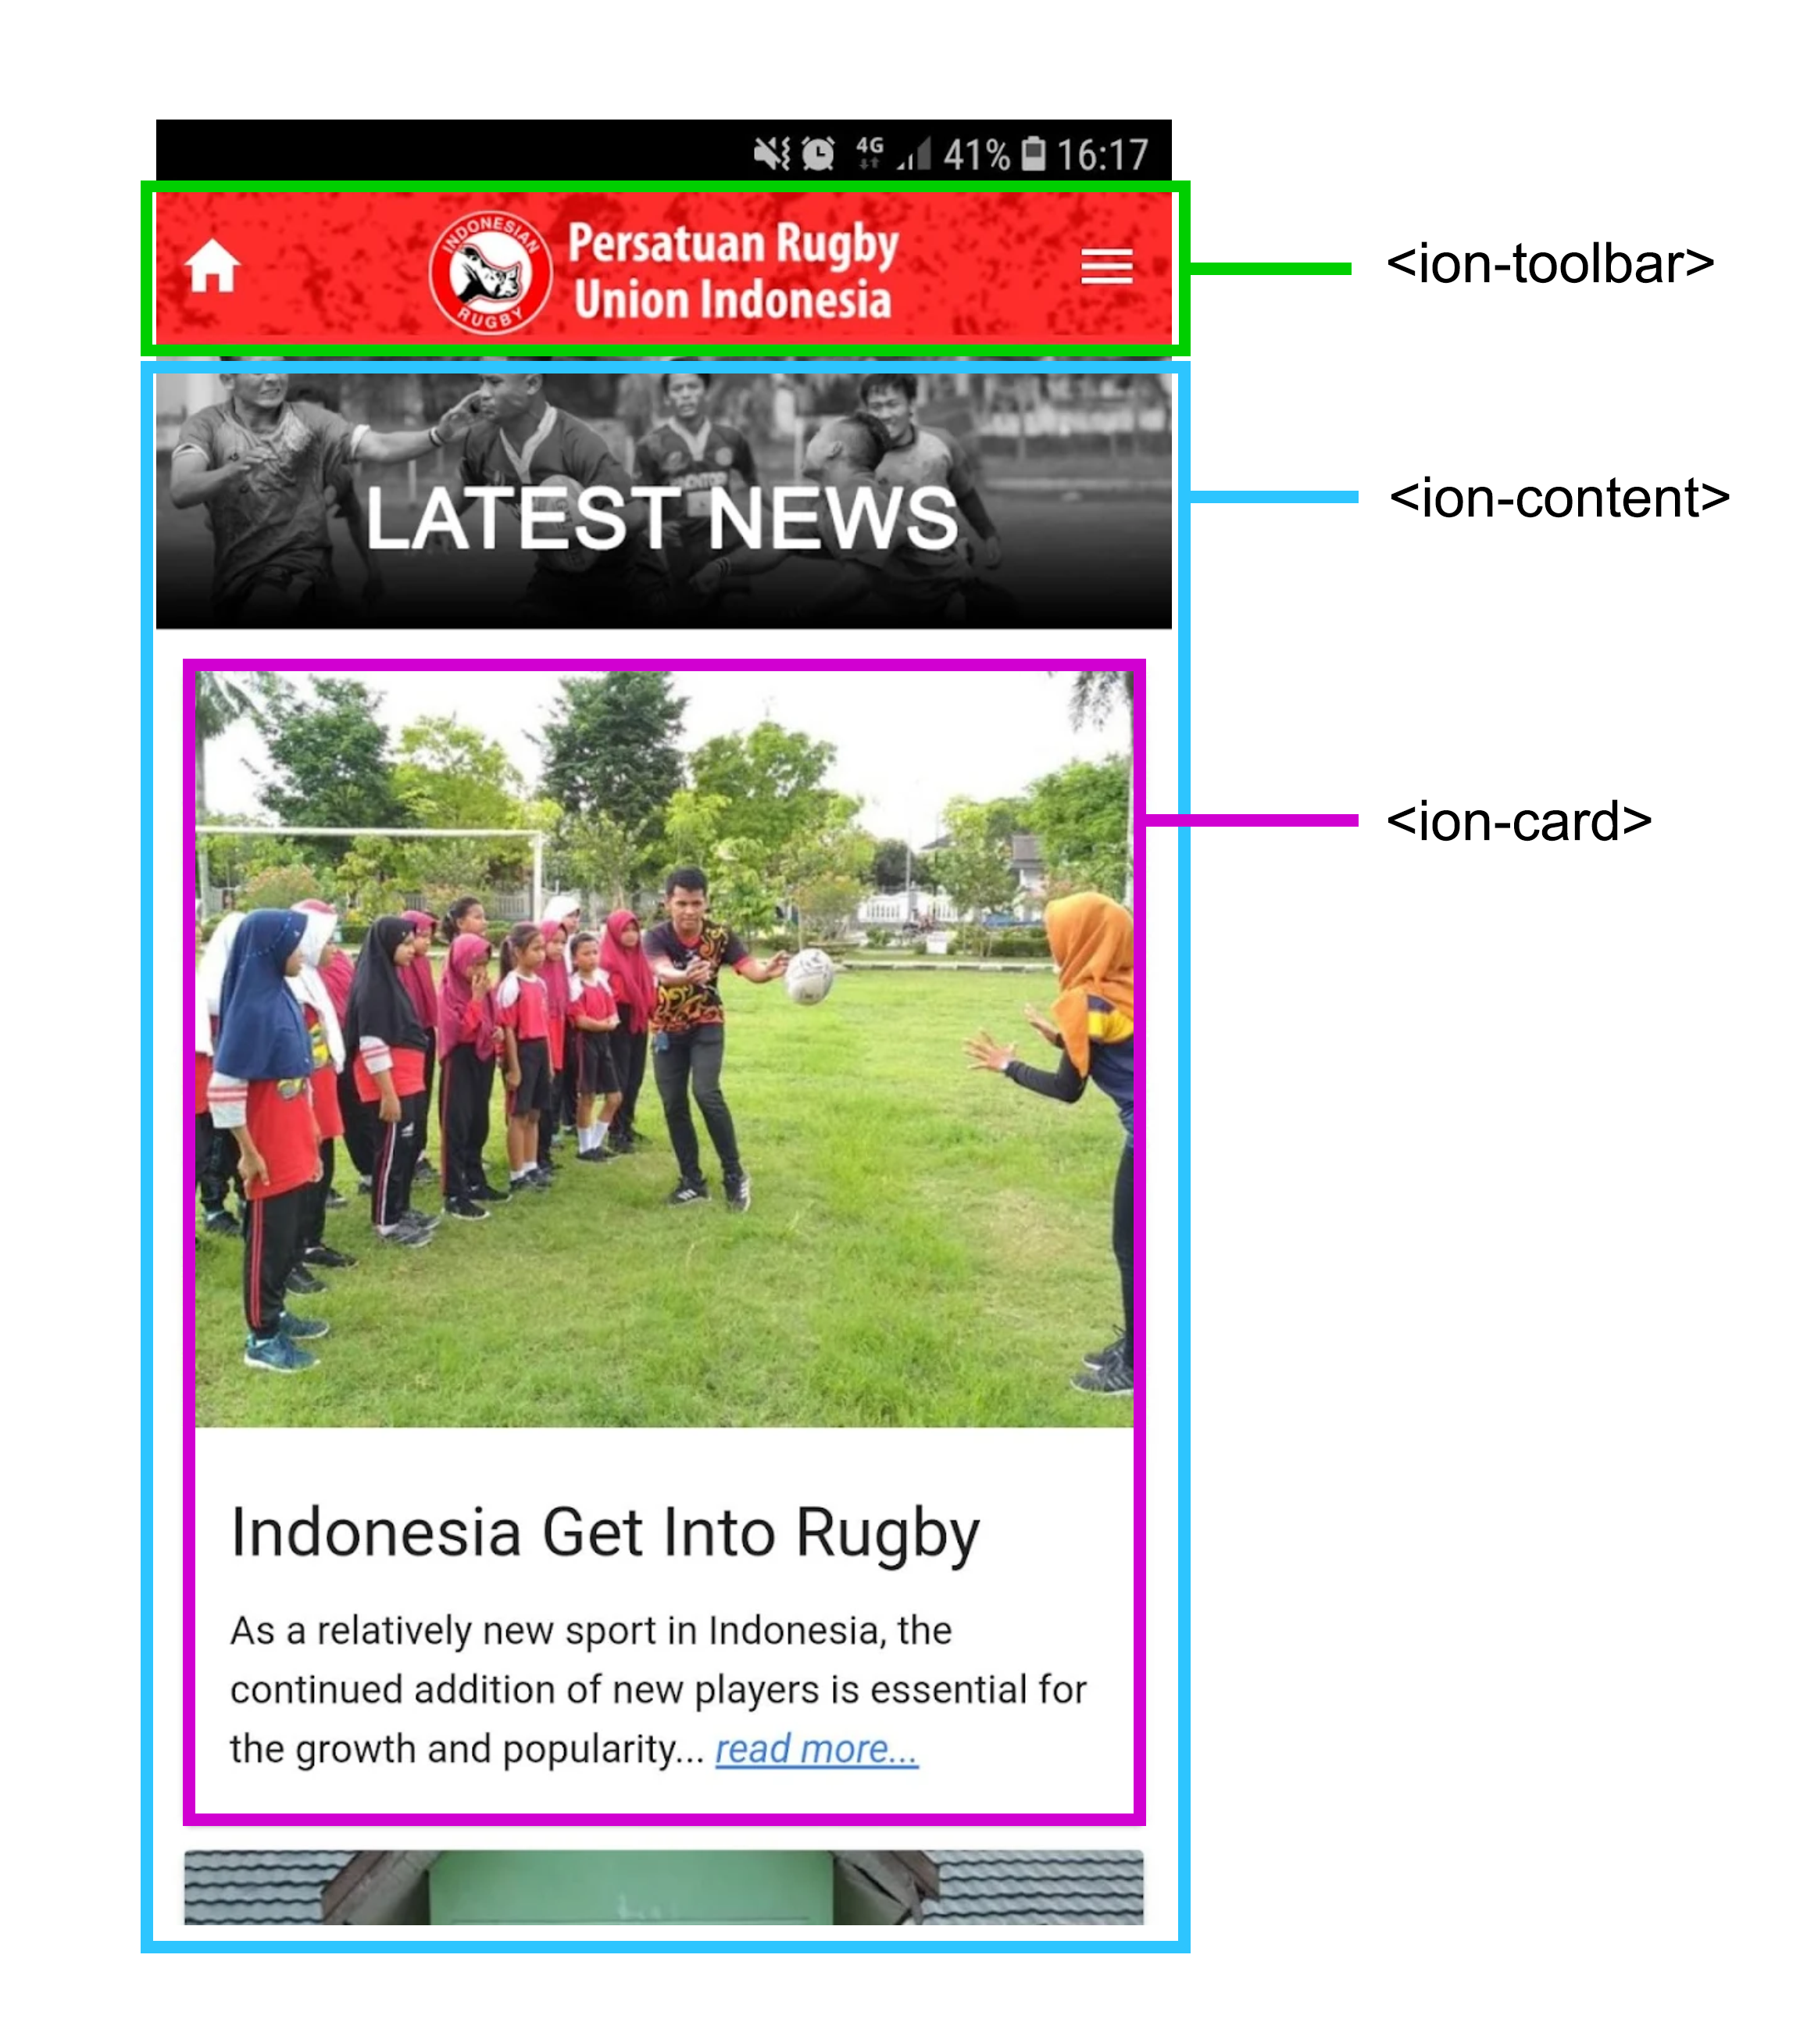
\includegraphics[scale=0.1]{Gambar/latest_news-analytics.png}
    \caption{Analisis dari Halaman Utama Rugby Indonesia}
    \label{fig:homepage-analytics}
\end{figure}

Pada saat aplikasi Rugby Indonesia dijalankan, secara default aplikasi akan membuka file main.tsx yang berada di app/src. File tersebut akan merender App.tsx untuk menjadi tampilan aplikasi. 

\begin{lstlisting}[language=HTML, caption=Kode dari main.tsx, label=kode:main-tsx]
import React from 'react';
import { createRoot } from 'react-dom/client';
import App from './App';
import { defineCustomElements } from '@ionic/pwa-elements/loader';

// Call the element loader before the render call
defineCustomElements(window);

const container = document.getElementById('root');
const root = createRoot(container!);
root.render(
  <React.StrictMode>
    <App />
  </React.StrictMode>
);
\end{lstlisting}

Pada kode tersebut [\ref{kode:main-tsx}], metode \texttt{defineCustomElements} dipanggil dengan parameter \texttt{window}. metode defineCustomElements berfungsi sebagai element loader. Kode \texttt{document.getElementById} \texttt{('root')} digunakan untuk mendapatkan elemen dengan id `root'. Kode \texttt{createRoot} digunakan untuk membuat root element di mana kode ini akan menerima elemen yang akan dijadikan root.

Kode \texttt{root.render} digunakan untuk merender aplikasi React di dalam root element yang sudah dibuat. Kode \texttt{<React.StrictMode>} digunakan untuk mengaktifkan Strict Mode. Ini membantu mendeteksi masalah pada waktu kompilasi dan memberikan peringatan tambahan saat pengembangan. Kode \texttt{<App />} adalah komponen utama yang dirender di dalam Strict Mode. Komponen ini yang akan merender file App.tsx.

Pada file App.tsx, file ini akan melakukan route ke tiap halaman menggunakan \texttt{IonRouteOutlet} [\ref{subbab:router}]. Secara default, route utama dari App.tsx akan menuju ke dalam \texttt{path="/folder/:name"} di mana path ini akan membuka Page.tsx. Pengembang dapat mengubah path dari route tersebut dengan path yang dibutuhkan.

\begin{lstlisting}[language=HTML, caption=Kode dari App.tsx, label=kode:app-tsx]
import { IonApp, IonRouterOutlet, IonSplitPane, setupIonicReact } from '@ionic/react';
import { IonReactRouter } from '@ionic/react-router';
import { Redirect, Route } from 'react-router-dom';
import Menu from './components/Menu';
import Page from './pages/Page';

/* Core CSS required for Ionic components to work properly */
import '@ionic/react/css/core.css';

/* Basic CSS for apps built with Ionic */
import '@ionic/react/css/normalize.css';
import '@ionic/react/css/structure.css';
import '@ionic/react/css/typography.css';

/* Optional CSS utils that can be commented out */
import '@ionic/react/css/padding.css';
import '@ionic/react/css/float-elements.css';
import '@ionic/react/css/text-alignment.css';
import '@ionic/react/css/text-transformation.css';
import '@ionic/react/css/flex-utils.css';
import '@ionic/react/css/display.css';

/* Theme variables */
import './theme/variables.css';

/* This import is for page */
import LatestNews from './pages/latest_news/latest_news';
import TeammatePhotos from './pages/teammate_photos/teammate_photos';

setupIonicReact();

const App: React.FC = () => {
  return (
    <IonApp>
      <IonReactRouter>
        <IonSplitPane contentId="main">
          <Menu />
          <IonRouterOutlet id="main">
            <Route path="/" exact={true}>
              <Redirect to="/latest_news" />
            </Route>
            <Route path="/latest_news" exact={true}>
              <LatestNews />
            </Route>
            <Route path="/teammate_photos" exact={true}>
              <TeammatePhotos />
            </Route>
            <Route path="/folder/:name" exact={true}>
              <Page />
            </Route>
          </IonRouterOutlet>
        </IonSplitPane>
      </IonReactRouter>
    </IonApp>
  );
};

export default App;

\end{lstlisting}

Pada kode tersebut [\ref{kode:app-tsx}], terdapat metode \texttt{setupIonicReact()} yang berguna untuk mengkonfigurasi Ionic agar bekerja dengan React. Komponen \texttt{IonSplitPane} pada kode berguna untuk memisahkan panel menu dengan halaman. Komponen \texttt{IonRouterOutlet} pada kode berguna untuk melakukan routing ke halaman yang diinginkan. Pada kode ini, secara default aplikasi akan membuka halaman `Latest News' dikarenakan ketika path bernilai "/", maka halaman yang dibuka adalah halaman Latest News.

Pada file latest\_news.tsx, file ini akan mengambil berita dari \url{https://rugbyindonesia.or.id/berita/} dan akan ditampilkan pada halaman Latest News. Setiap berita yang terdapat pada halaman Latest News akan ditampilkan menggunakan \texttt{IonCard}.

\begin{lstlisting}[language=HTML, caption=Kode dari latest\_news.tsx, label=kode:latest-news-tsx]
import { IonButtons, IonContent, IonHeader, IonMenuButton, IonPage, IonTitle, IonToolbar, IonBackButton, IonCard, IonCardHeader, IonCardTitle, IonCardContent} from '@ionic/react';
import './latest_news.css';

import bannerImage from '../../images/sub-header-news.png';
import latestNews1 from '../../images/latest_news_image_1.jpeg';
import homeIcon from '../../images/home_icon.png';

const Page: React.FC = () => {

    return (
        <IonPage>
            <IonHeader>
                <IonToolbar>
                    <IonButtons slot="start">
                        <a href='/latest_news'>
                            <div className='home-icon'>
                                <img src={homeIcon} alt="home-icon" />
                            </div>
                        </a> 
                    </IonButtons>
                    <IonButtons slot="end">
                        <IonMenuButton />
                    </IonButtons>
                    <IonTitle>
                        Persatuan Rugby
                        Union Indonesia
                    </IonTitle>
                </IonToolbar>
            </IonHeader>
            <IonContent className="ion-padding">
                <div className="news section">
                    <img src = {bannerImage} alt='latest-news-banner'/>
                </div>
                <IonCard>
                    <img alt='latest-news-image-1' src={latestNews1}/>
                    <IonCardHeader>
                        <IonCardTitle>Rugby Masuk Sekolah resmi dimulai di DKI Jakarta</IonCardTitle>
                    </IonCardHeader>

                    <IonCardContent>
                    Program Rugby Masuk Sekolah resmi dimulai di DKI Jakarta dengan serah terima Bola dan Baju Pelatih Rugby Masuk Sekolah dari PB PRUI ke PRUI DKI Jakarta pada Hari Sabtu, 25 November 2023 di Lapangan Pondok Bambu, Jakarta. Wakil Ketua II PB PRUI, Pak Agus Djamhoer menyerahkan paket Rugby Masuk Sekolah ini kepada Pak Tito Vau selaku Ketua PRUI DKI Jakarta pada acara Kejuaraan Daerah Rugby tingkat Pelajar DKI Jakarta. 
                    <br></br><br></br>
                    DKI Jakarta memiliki 17 pelatih yang sudah mengikuti sertifikasi pelatih Rugby Masuk Sekolah dan siap mengajarkan T1 Rugby ke seluruh tingkatan sekolah di Jakarta. Pada saat ini tercatat sudah lebih dari 13 sekolah di Jakarta dan jumlah sekolah ini akan terus ditingkatkan seiring dengan waktu program ini berjalan.
                    </IonCardContent>
                </IonCard>
            </IonContent>
        </IonPage>
    );
};

export default Page;
\end{lstlisting}

Kode ini \ref{kode:latest-news-tsx} akan menampilkan halaman Latest News yang memiliki komponen toolbar, button, content, dan card. Content dari halaman ini berisi berita-berita yang terdapat pada \url{https://rugbyindonesia.or.id/berita/}.

\subsection{Halaman Teammate Photos}
Pada halaman Teammate Photos, skenario dari aplikasi Rugby Indonesia sama dengan skenario dari halaman Teammate Photos yang sudah ada [\ref{tab:existing-scenario-teammate-photos-page}], namun dengan adanya sedikit penambahan, yaitu skenario di saat pengguna mengupload gambar.
Penambahan ini dilakukan karena peneliti tidak menemukan gambar di saat pengguna mengunggah gambar.

\begin{table} [H]
    \centering
    \caption{Tabel Skenario saat Pengguna Mengupload Gambar}
    \begin{tabular}{|c|c|c|}
    \hline
       No. & Aksi Aktor & Reaksi Sistem  \\ \hline
        1 & Pengguna menekan tombol  & Aplikasi akan membuka kamera \\
         & ``Take a Photo''. & pada \textit{smartphone}. \\ \hline
        2 & Pengguna mengambil gambar & Aplikasi akan menampilkan \\ 
         & dari kamera. & Cards yang berisi frame \\ \hline
        3 & Pengguna memilih salah satu frame & Aplikasi akan menampilkan \\ 
         & lalu mengklik tombol ``OK'' & konfirmasi \\ \hline
        4 & Pengguna mengklik & Sistem akan mengunggah gambar \\ 
         & tombol ``YA'' & ke dalam aplikasi. \\ \hline
    \end{tabular}
    \label{tab:usulan-skenario-halaman-teammate-photos}
\end{table}

Skenario tersebut [\ref{tab:usulan-skenario-halaman-teammate-photos}] juga berlaku ketika pengguna menekan tombol ``LOAD FROM LIBRARY'', hanya saja perbedaannya terdapat pada reaksi sistem, yaitu Aplikasi akan membuka gallery dari smartphone pengguna.

Pada halaman Teammate Photos, terdapat beberapa komponen dari Ionic 7 yang digunakan. Halaman ini memiliki beberapa komponen, yaitu toolbar, button, content, dan juga card.

\begin{figure} [H]
    \centering
    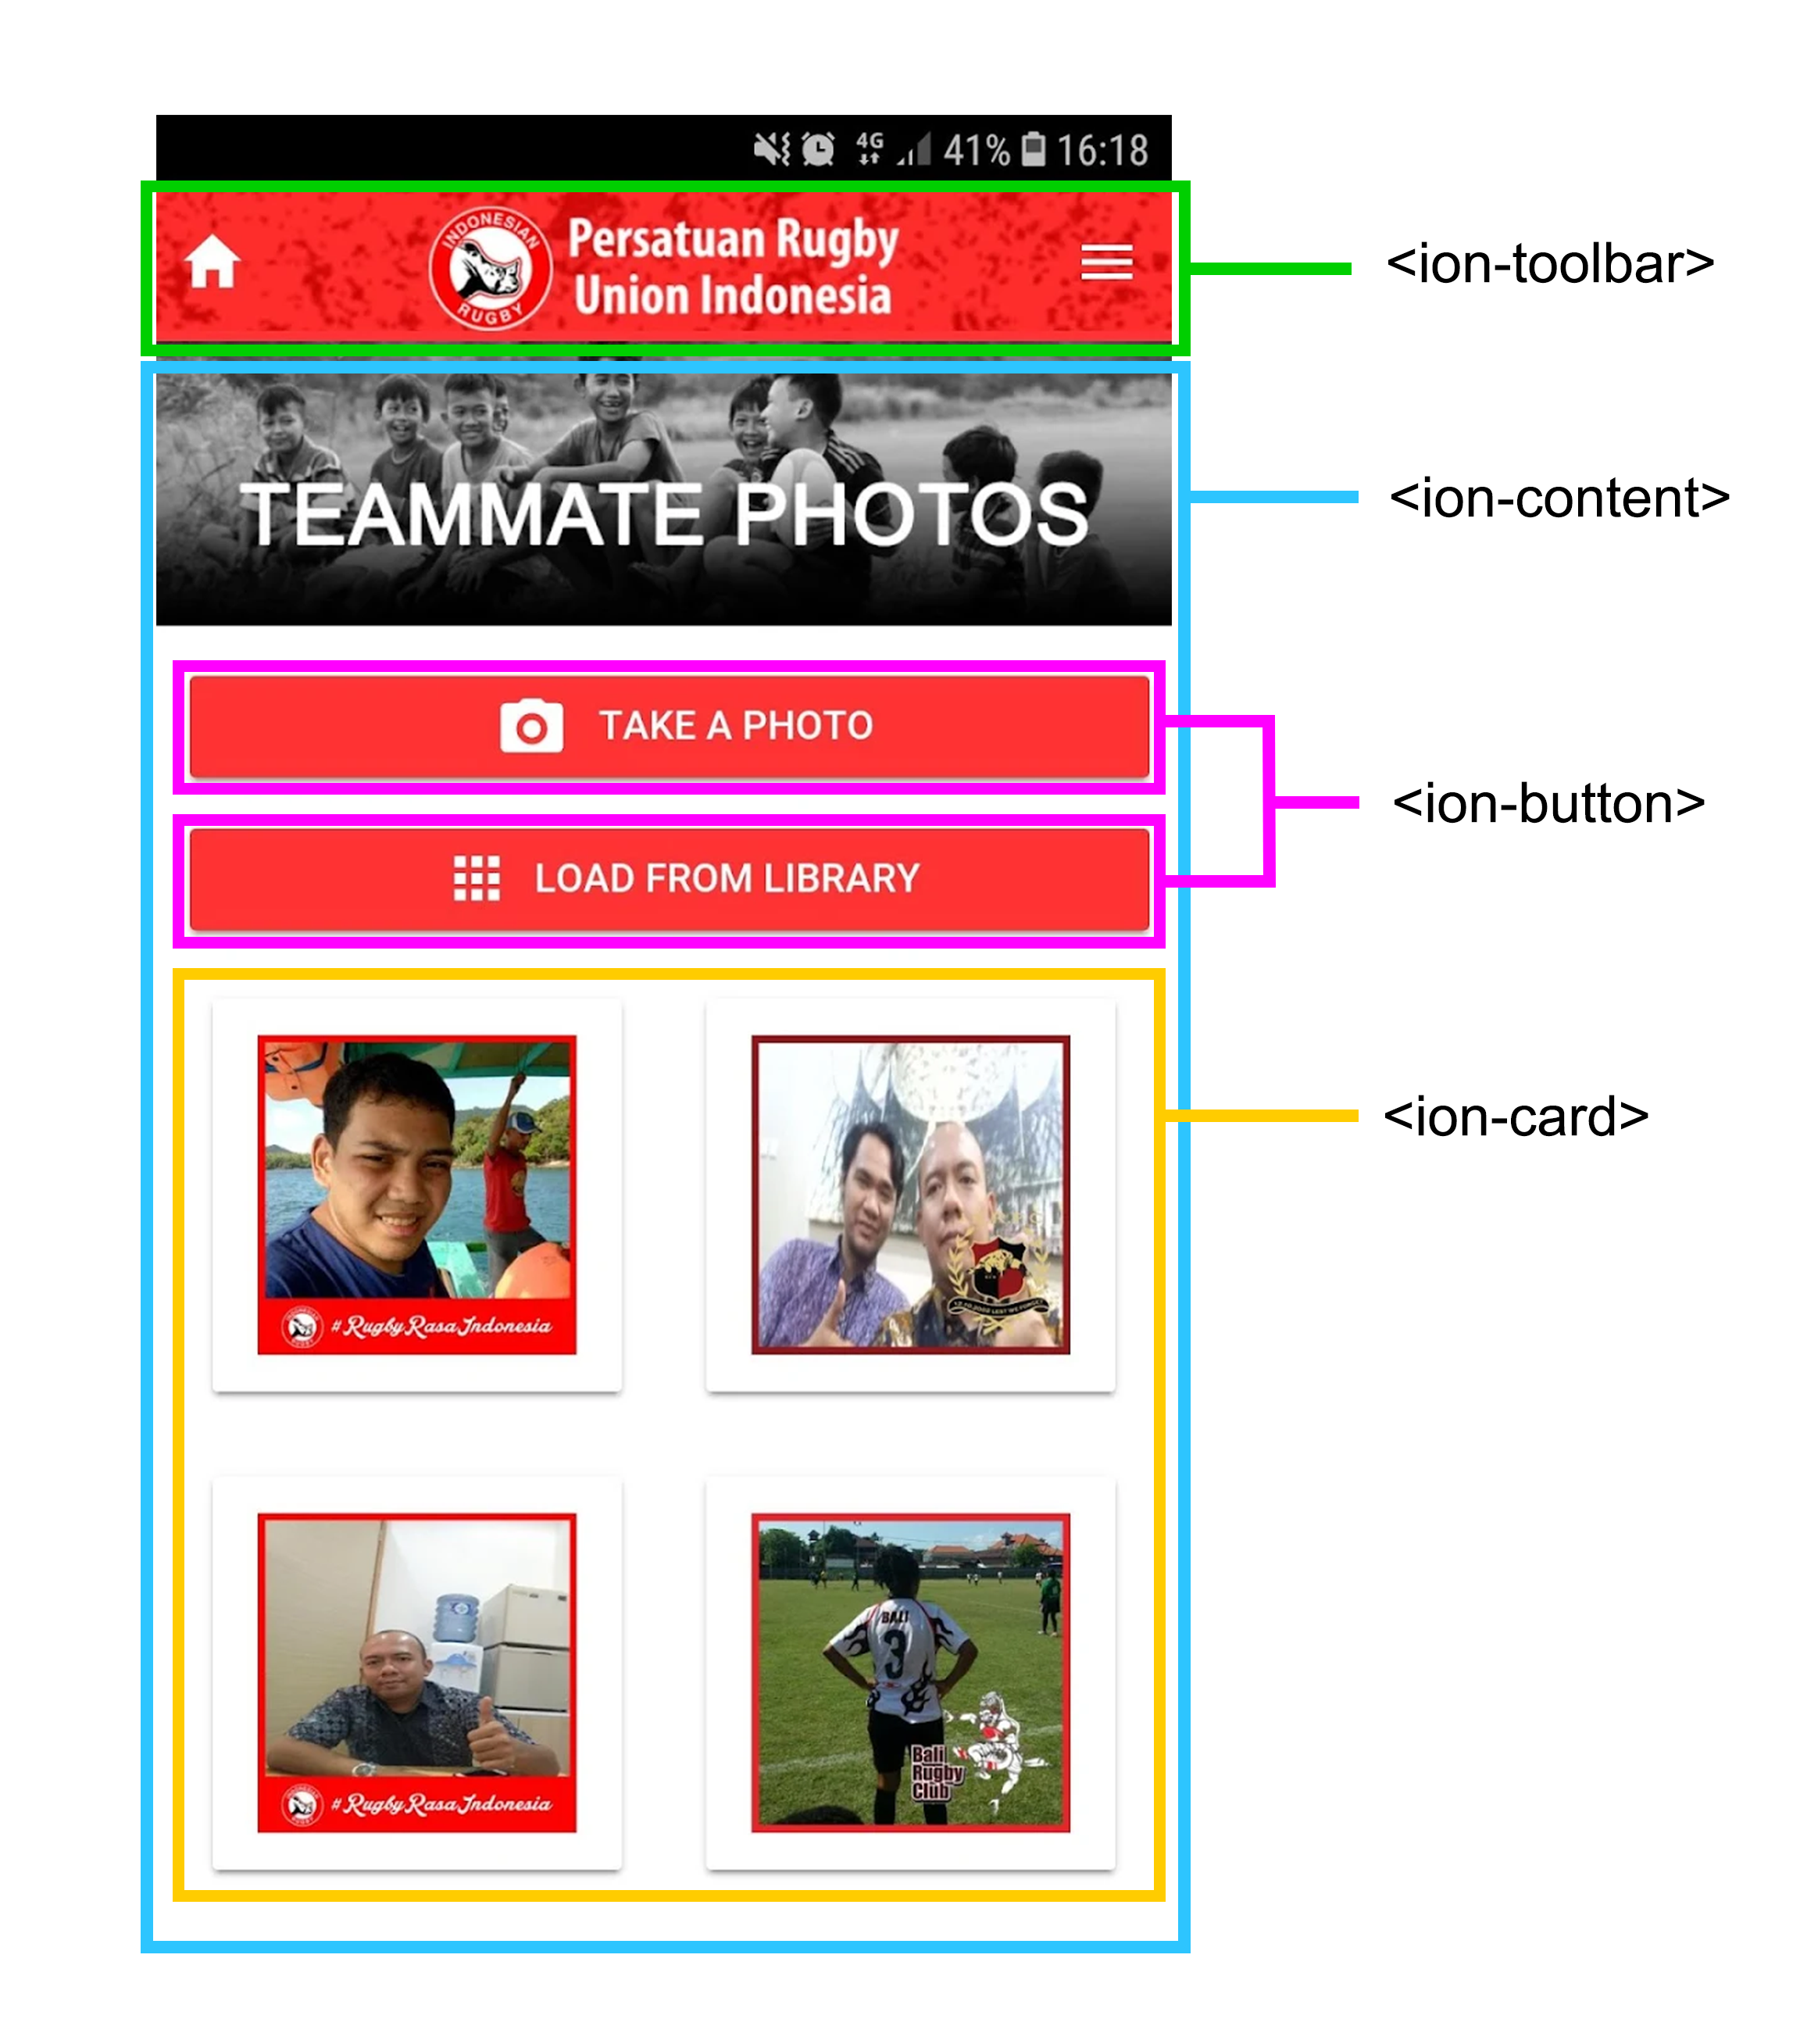
\includegraphics[scale=0.1]{Gambar/teammates_photos-analytics.png}
    \caption{Analisis dari Halaman Teammate Photos}
    \label{fig:teammate-photos-analytics}
\end{figure}

Pada saat pengguna memilih menu Teammate Photos, aplikasi akan menjalankan file teammate\_photos.tsx. File ini memiliki fungsi untuk menangkap gambar, dan melihat hasil tangkapan gambar milik pengguna tersebut atau pun orang lain.

\begin{lstlisting}[language=HTML, caption=Kode dari teammate\_photos.tsx, label=kode:teammate-photos-tsx]
import React, { useState } from 'react';
import { IonButtons, IonContent, IonHeader, IonMenuButton, IonPage, IonTitle, IonToolbar, IonBackButton, IonButton, IonIcon} from '@ionic/react';
import { Camera, Photo, CameraResultType, CameraSource } from '@capacitor/camera';
import { Directory, Filesystem } from '@capacitor/filesystem';

import './teammate_photos.css';

import bannerImage from '../../images/sub-header-photo.png';
import homeIcon from '../../images/home_icon.png';

import { PhotoImages } from "./photoImages";
import PhotoGallery from './photoGallery';
import { appsSharp, camera, menuSharp } from 'ionicons/icons';

const Page: React.FC = () => {
    const [images, setImages] = useState<PhotoImages[]>([]);

    const takePicture = async () => {
        const image = await Camera.getPhoto({
            quality: 90,
            allowEditing: true,
            resultType: CameraResultType.Uri
        });
    
        const fileName = new Date().getTime() + '.jpeg';
        
        const savedFileImage = await savePicture(image, fileName);
        var imageUrl = savedFileImage.filePath!;
        console.log(imageUrl);
        // Can be set to the src of an image now
        // imageElement.src = imageUrl;
        setImages([...images, savedFileImage]);

    };

    const savePicture = async(photo: Photo, fileName: string):Promise<PhotoImages> => {
        let base64data:string;
        base64data = await base64FromPath(photo.webPath!);

        const savedPicture = await Filesystem.writeFile({
            path: fileName,
            directory: Directory.Data,
            data: base64data
        });

        return{
            filePath: fileName,
            webviewPath: photo.webPath
        }
    }

    async function base64FromPath(path:string): Promise<string>{
        const response = await fetch(path);
        const blob = await response.blob();

        return new Promise((resolve, reject) => {
            const reader = new FileReader();
            reader.onerror = reject;
            reader.onload = () => {
                if (typeof reader.result === 'string')
                {
                    resolve(reader.result);
                }
                else
                {
                    reject('This method did not return a string');
                }
            };

            reader.readAsDataURL(blob);
        })
    }

    return (
        <IonPage>
            <IonHeader>
                <IonToolbar>
                    <IonButtons slot="start">
                        <a href='/latest_news'>
                            <div className='home-icon'>
                                <img src={homeIcon} alt="home-icon" />
                            </div>
                        </a>                     
                    </IonButtons>
                    <IonButtons slot="end">
                        <IonMenuButton />
                    </IonButtons>
                    <IonTitle>
                        Persatuan Rugby
                        Union Indonesia
                    </IonTitle>
                </IonToolbar>
            </IonHeader>
            <IonContent className="ion-padding">
                <div className='teammate-photos-banner'>
                    <img src={bannerImage} alt="Teammate-Photos-Banner" />
                </div>
                <br></br>
                <IonButton color="primary" expand='block' onClick={onClick => takePicture()}>
                    <IonIcon slot="start" icon={camera}></IonIcon>
                    Take Photo
                </IonButton> {/* Use the onClick prop directly */}

                <IonButton color='primary' expand='block'>
                    <IonIcon slot="start" icon={appsSharp}></IonIcon>
                    Load from Library
                </IonButton>

                <PhotoGallery photos={images} />
            </IonContent>
        </IonPage>
    );
};

export default Page;

\end{lstlisting}

Pada kode tersebut [\ref{kode:teammate-photos-tsx}], kode \texttt{const [images, setImages] = useState<PhotoImages[]>} \texttt{([]);} menggunakan useState untuk menyimpan daftar foto yang diambil dalam bentuk objek PhotoImages. Fungsi \texttt{takePicture} menggunakan Capacitor Camera untuk mengambil foto. 

\begin{lstlisting}[language=HTML, caption=Kode dari photoImages.tsx, label=kode:photo-image-tsx]
export interface PhotoImages
{
    filePath: string;
    webviewPath?: string;
}

\end{lstlisting}

\begin{lstlisting}[language=HTML, caption=Kode dari photoGallery.tsx, label=kode:photo-gallery-tsx]
import { IonCol, IonGrid, IonImg, IonRow } from "@ionic/react";
import { PhotoImages } from "./photoImages";
import React from "react";

type Props = {
    photos: PhotoImages[],
}

const PhotoGallery: React.FC<Props> =({photos}) => {
    return (
        <IonGrid>
            <IonRow>
                {photos.map((photo, idx) =>(
                    <IonCol size = "6" key={idx}>
                        <IonImg src={photo.webviewPath}/>
                    </IonCol>
                ))}
            </IonRow>
        </IonGrid>
    );
}

export default PhotoGallery;
\end{lstlisting}